\subsection{Building the kernel}

\subsection{Kernel configuration}

\begin{frame}
  \frametitle{Kernel configuration}
  \begin{itemize}
  \item The kernel contains thousands of device drivers, filesystem
    drivers, network protocols and other configurable items
  \item Thousands of options are available, that are used to
    selectively compile parts of the kernel source code
  \item The kernel configuration is the process of defining the set of
    options with which you want your kernel to be compiled
  \item The set of options depends
    \begin{itemize}
    \item On the target architecture and on your hardware (for device drivers, etc.)
    \item On the capabilities you would like to give to your kernel
      (network capabilities, filesystems, real-time, etc.).
      Such generic options are available in all architectures.
    \end{itemize}
  \end{itemize}
\end{frame}

\begin{frame}
  \frametitle{Specifying the target architecture}
  First, specify the architecture for the kernel to build
  \begin{itemize}
  \item Set it to the name of a directory under \kdir{arch}:\\
  	\code{export ARCH=arm}
  \item By default, the kernel build system assumes that the
        kernel is configured and built for the host architecture
	(\code{x86} in our case, native kernel compiling)
  \item The kernel build system will use this setting to:
  	\begin{itemize}
	\item Use the configuration options for the target
	      architecture.
	\item Compile the kernel with source code and headers
	      for the target architecture.
	\end{itemize}
  \end{itemize}
\end{frame}

\begin{frame}
  \frametitle{Kernel configuration and build system}
  \begin{itemize}
  \item The kernel configuration and build system is based on multiple
    Makefiles
  \item One only interacts with the main \kfile{Makefile}, present at
    the {\bf top directory} of the kernel source tree
  \item Interaction takes place
    \begin{itemize}
    \item using the \code{make} tool, which parses the Makefile
    \item through various {\bf targets}, defining which action should
      be done (configuration, compilation, installation, etc.). Run
      \code{make help} to see all available targets.
    \end{itemize}
  \item Example
    \begin{itemize}
    \item \code{cd linux-4.14.x/}
    \item \code{make <target>}
    \end{itemize}
  \end{itemize}
\end{frame}

\begin{frame}
  \frametitle{Kernel configuration details}
  \begin{itemize}
  \item The configuration is stored in the \code{.config} file at the
    root of kernel sources
    \begin{itemize}
    \item Simple text file, \code{CONFIG_PARAM=value} (included by the kernel Makefile)
    \end{itemize}
  \item As options have dependencies, typically never edited by hand,
    but through graphical or text interfaces:
    \begin{itemize}
    \item \code{make xconfig}, \code{make gconfig} (graphical)
    \item \code{make menuconfig}, \code{make nconfig} (text)
    \item You can switch from one to another, they all load/save the
      same \code{.config} file, and show the same set of options
    \end{itemize}
  \end{itemize}
\end{frame}

\begin{frame}
  \frametitle{Initial configuration}
  Difficult to find which kernel configuration will work
  with your hardware and root filesystem. Start with one
  that works!
  \begin{itemize}
  \item Desktop or server case:
     \begin{itemize}
       \item Advisable to start with the configuration of your running
	  kernel, usually available in \code{/boot}:\\
	  \code{cp /boot/config-`uname -r` .config}
     \end{itemize}
  \item Embedded platform case:
     \begin{itemize}
  	\item Default configuration files are available, usually for
	  each CPU family.
        \item They are stored in \code{arch/<arch>/configs/}, and are
          just minimal \code{.config} files (only settings different
          from default ones).
        \item Run \code{make help} to find if one is available for your
          platform
        \item To load a default configuration file, just run\\
          \code{make cpu_defconfig}
        \item This will overwrite your existing \code{.config} file!
     \end{itemize}
  \end{itemize}
  Now, you can make configuration changes (\code{make menuconfig}...).
\end{frame}

\begin{frame}
  \frametitle{Create your own default configuration}
  To create your own default configuration file:
  \begin{itemize}
     \item \code{make savedefconfig}\\
       This creates a minimal configuration (non-default settings)
     \item \code{mv defconfig arch/<arch>/configs/myown_defconfig}\\
       This way, you can share a reference configuration inside
       the kernel sources. 
  \end{itemize}
\end{frame}

\begin{frame}
  \frametitle{Kernel or module?}
  \begin{itemize}
  \item The {\bf kernel image} is a {\bf single file}, resulting from
    the linking of all object files that correspond to features
    enabled in the configuration
    \begin{itemize}
    \item This is the file that gets loaded in memory by the
      bootloader
    \item All included features are therefore available as soon as the
      kernel starts, at a time where no filesystem exists
    \end{itemize}
  \item Some features (device drivers, filesystems, etc.) can however
    be compiled as {\bf modules}
    \begin{itemize}
    \item These are {\em plugins} that can be loaded/unloaded dynamically to
      add/remove features to the kernel
    \item Each {\bf module is stored as a separate file in the
        filesystem}, and therefore access to a filesystem is mandatory
      to use modules
    \item This is not possible in the early boot procedure of the
      kernel, because no filesystem is available
    \end{itemize}
  \end{itemize}
\end{frame}

\begin{frame}
  \frametitle{Kernel option types}
  There are different types of options
  \begin{itemize}
  \item \code{bool} options, they are either
    \begin{itemize}
    \item {\em true} (to include the feature in the kernel) or
    \item {\em false} (to exclude the feature from the kernel)
    \end{itemize}
  \item \code{tristate} options, they are either
    \begin{itemize}
    \item {\em true} (to include the feature in the kernel image) or
    \item {\em module} (to include the feature as a kernel module) or
    \item {\em false} (to exclude the feature)
    \end{itemize}
  \item \code{int} options, to specify integer values
  \item \code{hex} options, to specify hexadecimal values
  \item \code{string} options, to specify string values
  \end{itemize}
\end{frame}

\begin{frame}
  \frametitle{Kernel option dependencies}
  \begin{itemize}
  \item There are dependencies between kernel options
  \item For example, enabling a network driver requires the network
    stack to be enabled
  \item Two types of dependencies
    \begin{itemize}
    \item \code{depends on} dependencies. In this case, option B that
      depends on option A is not visible until option A is enabled
    \item \code{select} dependencies. In this case, with option B
      depending on option A, when option A is enabled, option B is
      automatically enabled. In particular, such dependencies are
      used to declare what features a hardware architecture supports.
    \end{itemize}
  \item With the \code{Show All Options} option, \code{make xconfig} allows
    to see all options, even the ones that cannot be selected because of
    missing dependencies. Values for dependencies are shown.
  \end{itemize}
\end{frame}

\begin{frame}
  \frametitle{make xconfig}
  \code{make xconfig}
  \begin{itemize}
  \item The most common graphical interface to configure the kernel.
  \item Make sure you read\\
    \code{help ->  introduction: useful options!}
  \item File browser: easier to load configuration files
  \item Search interface to look for parameters
  \item Required Debian / Ubuntu packages: \code{qt5-default}
  \end{itemize}
\end{frame}

\begin{frame}
  \frametitle{make xconfig screenshot}
  \begin{center}
    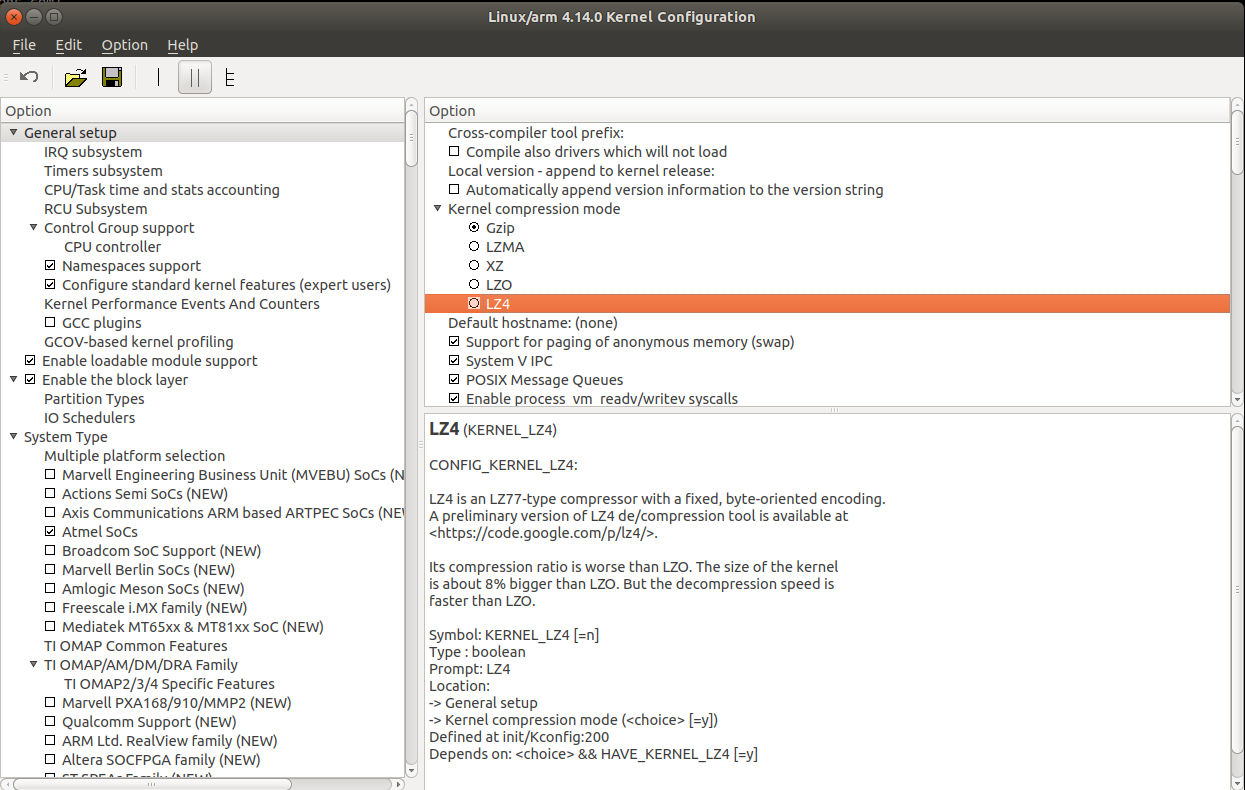
\includegraphics[height=0.8\textheight]{slides/sysdev-kernel-building/xconfig-screenshot.png}
  \end{center}
\end{frame}

\begin{frame}
  \frametitle{make xconfig search interface}

  Looks for a keyword in the parameter name. Allows to select or
  unselect found parameters.

  \begin{center}
    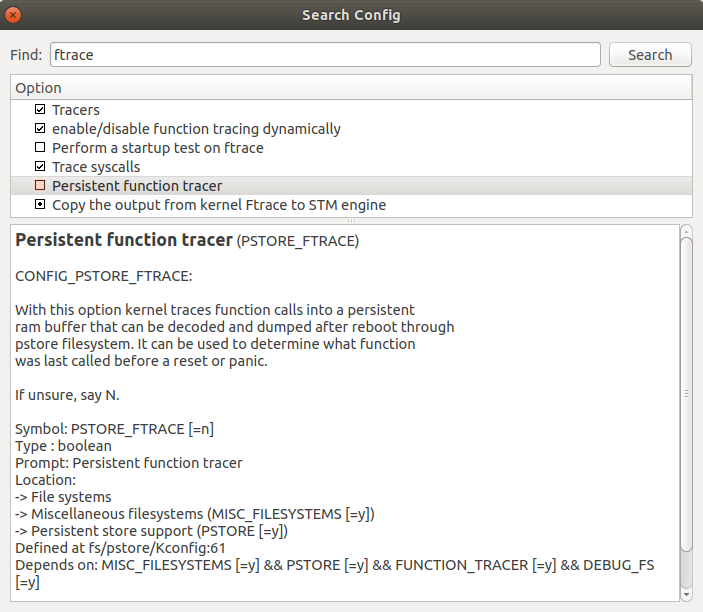
\includegraphics[height=0.7\textheight]{slides/sysdev-kernel-building/xconfig-search.png}
  \end{center}
\end{frame}

\begin{frame}
\frametitle{Kernel configuration options}
  \begin{center}
    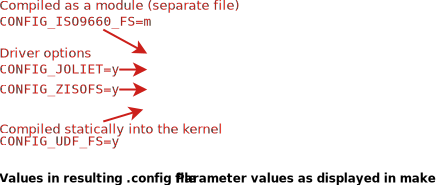
\includegraphics[width=\textwidth]{slides/sysdev-kernel-building/xconfig-iso-example.pdf}
  \end{center}
\end{frame}

\begin{frame}[fragile]
  \frametitle{Corresponding .config file excerpt}
  Options are grouped by sections and are prefixed with
  \code{CONFIG_}.
\footnotesize
\begin{verbatim}
#
# CD-ROM/DVD Filesystems
#
CONFIG_ISO9660_FS=m
CONFIG_JOLIET=y
CONFIG_ZISOFS=y
CONFIG_UDF_FS=y
CONFIG_UDF_NLS=y

#
# DOS/FAT/NT Filesystems
#
# CONFIG_MSDOS_FS is not set
# CONFIG_VFAT_FS is not set
CONFIG_NTFS_FS=m
# CONFIG_NTFS_DEBUG is not set
CONFIG_NTFS_RW=y
\end{verbatim}
\end{frame}

\begin{frame}
  \frametitle{make gconfig}
  \begin{columns}
    \column{0.5\textwidth}
    \code{make gconfig}
    \begin{itemize}
      \item {\em GTK} based graphical configuration interface. Functionality
            similar to that of make \code{xconfig}.
      \item Just lacking a search functionality.
      \item Required Debian packages: \code{libglade2-dev}
    \end{itemize}
    \column{0.5\textwidth}
    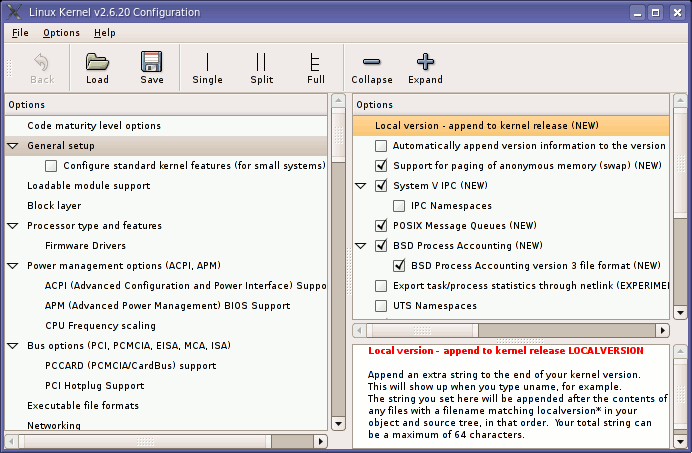
\includegraphics[width=\textwidth]{slides/sysdev-kernel-building/gconfig-screenshot.png}
  \end{columns}
\end{frame}

\begin{frame}
  \frametitle{make menuconfig}
  \begin{columns}
    \column{0.5\textwidth}
    \code{make menuconfig}
    \begin{itemize}
      \item Useful when no graphics are available. Pretty convenient too!
      \item Same interface found in other tools: BusyBox, Buildroot...
      \item Required Debian packages: \code{libncurses-dev}
    \end{itemize}
    \column{0.5\textwidth}
    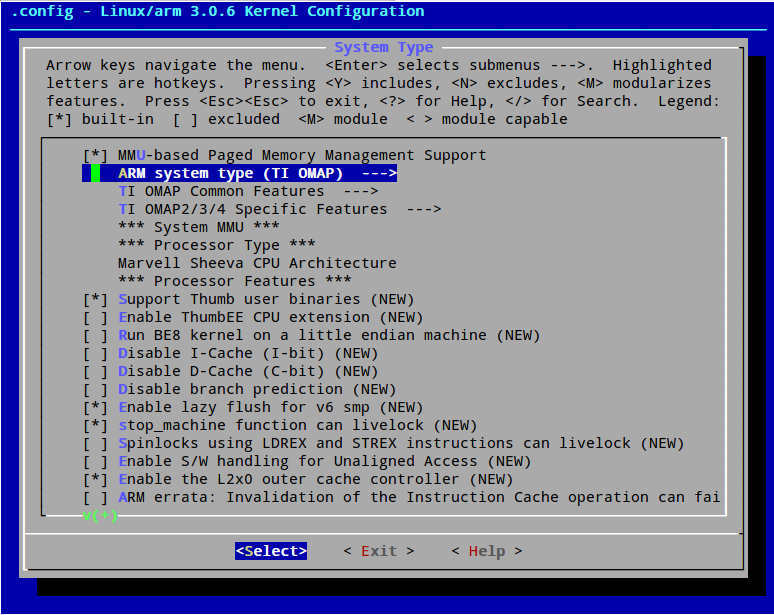
\includegraphics[width=\textwidth]{slides/sysdev-kernel-building/menuconfig-screenshot.png}
  \end{columns}
\end{frame}

\begin{frame}
  \frametitle{make nconfig}
  \begin{columns}
    \column{0.5\textwidth}
    \code{make nconfig}
    \begin{itemize}
      \item A newer, similar text interface
      \item More user friendly (for example, easier to access help information).
      \item However, lacking the shortcuts that \code{menuconfig} offers
	in search results. Therefore, much less convenient than \code{menuconfig}.
      \item Required Debian packages: \code{libncurses-dev}
    \end{itemize}
    \column{0.5\textwidth}
    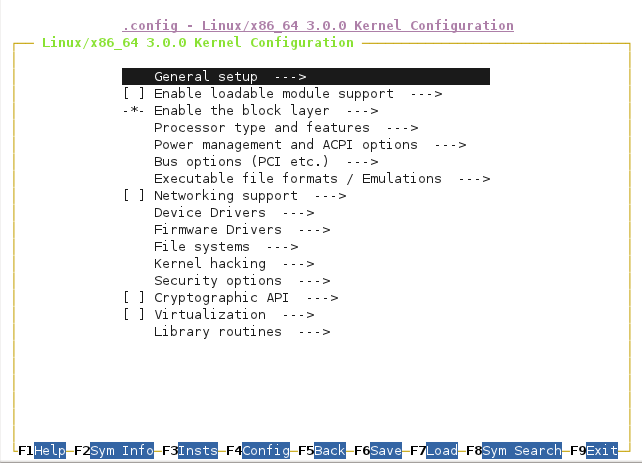
\includegraphics[width=\textwidth]{slides/sysdev-kernel-building/nconfig-screenshot.png}
  \end{columns}
\end{frame}

\begin{frame}
  \frametitle{make oldconfig}
  \code{make oldconfig}
  \begin{itemize}
  \item Needed very often!
  \item Useful to upgrade a \code{.config} file from an earlier kernel release
  \item silently set default values for new parameters.
  \item Asks for values for new parameters.
  \end{itemize}
  If you edit a \code{.config} file by hand, it's useful
  to run \code{make oldconfig} afterwards, to set values to new
  parameters that could have appeared because of dependency changes.
\end{frame}

\begin{frame}
  \frametitle{Undoing configuration changes}
  A frequent problem:
  \begin{itemize}
  \item After changing several kernel configuration settings, your
    kernel no longer works.
  \item If you don't remember all the changes you made,
    you can get back to your previous configuration:\\
    \code{$ cp .config.old .config}
  \item All the configuration interfaces of the kernel
    (\code{xconfig}, \code{menuconfig}, \code{oldconfig}...) keep
    this \code{.config.old} backup copy.
  \end{itemize}
\end{frame}

\subsection{Compiling and installing the kernel}

\begin{frame}
  \frametitle{Choose a compiler}
  The compiler invoked by the kernel Makefile is \code{$(CROSS_COMPILE)gcc}
  \begin{itemize}
    \item When compiling natively
      \begin{itemize}
	 \item Leave \code{CROSS_COMPILE} undefined and the kernel
	    will be natively compiled for the host architecture
            using \code{gcc}.
      \end{itemize}
    \item When using a cross-compiler
      \begin{itemize}
      \item To make the difference with a native compiler, cross-compiler
          executables are prefixed by the name of the target system,
          architecture and sometimes library. Examples:\\
          \small
          \code{mips-linux-gcc}: the prefix is \code{mips-linux-}\\
          \code{arm-linux-gnueabi-gcc}: the prefix is \code{arm-linux-gnueabi-}
      \item So, you can specify your cross-compiler as follows:\\
          \code{export CROSS_COMPILE=arm-linux-gnueabi-}
      \end{itemize} 
  \end{itemize}
  \code{CROSS_COMPILE} is actually the prefix of the cross compiling
tools (\code{gcc}, \code{as}, \code{ld}, \code{objcopy}, \code{strip}...).
\end{frame}

\begin{frame}
  \frametitle{Specifying ARCH and CROSS\_COMPILE}
  There are actually two ways of defining \code{ARCH} and \code{CROSS_COMPILE}:
  \begin{itemize}
  \item Pass \code{ARCH} and \code{CROSS_COMPILE} on the \code{make}
    command line: \\
    \code{make ARCH=arm CROSS_COMPILE=arm-linux- ...} \\
    Drawback: it is easy to forget to pass these variables when
    you run any \code{make} command, causing your build and
    configuration to be screwed up.
  \item Define \code{ARCH} and \code{CROSS_COMPILE} as environment
    variables: \\
    \code{export ARCH=arm} \\
    \code{export CROSS_COMPILE=arm-linux-} \\
    Drawback: it only works inside the current
    shell or terminal. You could put these settings in a file
    that you source every time you start working on the project.
    If you only work on a single architecture with always the
    same toolchain, you could even put these settings in your
    \code{~/.bashrc} file to make them permanent and visible from
    any terminal.
  \end{itemize}
\end{frame}

\begin{frame}
  \frametitle{Kernel compilation}
  \begin{itemize}
  \item \code{make}
    \begin{itemize}
    \item In the main kernel source directory!
    \item Remember to run multiple jobs in parallel
          if you have multiple CPU cores. Example: \code{make -j 8}
    \item No need to run as root!
    \end{itemize}
  \item Generates
    \begin{itemize}
    \item \code{vmlinux}, the raw uncompressed kernel image, in the
      ELF format, useful for debugging purposes, but cannot be booted
    \item \code{arch/<arch>/boot/*Image}, the final, usually
      compressed, kernel image that can be booted
      \begin{itemize}
      \item \code{bzImage} for x86, \code{zImage} for ARM,
      \code{vmlinux.bin.gz} for ARC, etc.
      \end{itemize}
    \item \code{arch/<arch>/boot/dts/*.dtb}, compiled Device Tree
      files (on some architectures)
    \item All kernel modules, spread over the kernel source tree, as
      \code{.ko} ({\em Kernel Object}) files.
    \end{itemize}
  \end{itemize}
\end{frame}

\begin{frame}
  \frametitle{Kernel installation: native case}
  \begin{itemize}
  \item \code{make install}
    \begin{itemize}
    \item Does the installation for the host system by default, so
      needs to be run as root.
    \end{itemize}
  \item Installs
    \begin{itemize}
    \item \code{/boot/vmlinuz-<version>} \\
      Compressed kernel image. Same as the one in
      \code{arch/<arch>/boot}
    \item \code{/boot/System.map-<version>}\\
      Stores kernel symbol addresses for debugging purposes
      (obsolete: such information is usually stored in the kernel itself)
    \item \code{/boot/config-<version>}\\
      Kernel configuration for this version
    \end{itemize}
  \item In GNU/Linux distributions, typically re-runs the bootloader configuration
    utility to make the new kernel available at the next boot.
  \end{itemize}
\end{frame}

\begin{frame}
  \frametitle{Kernel installation: embedded case}
  \begin{itemize}
  \item \code{make install} is rarely used in embedded development, as the
    kernel image is a single file, easy to handle.
  \item Another reason is that there is no standard way to deploy and
    use the kernel image.
  \item Therefore making the kernel image available to the target is
    usually manual or done through scripts in build systems.
  \item It is however possible to customize the \code{make install}
    behavior in \code{arch/<arch>/boot/install.sh}
  \end{itemize}
\end{frame}

\begin{frame}
  \frametitle{Module installation: native case}
  \begin{itemize}
  \item \code{make modules_install}
    \begin{itemize}
    \item Does the installation for the host system by default, so
      needs to be run as root
    \end{itemize}
  \item Installs all modules in \code{/lib/modules/<version>/}
    \begin{itemize}
    \item \code{kernel/}\\
      Module \code{.ko} (Kernel Object) files, in the same directory
      structure as in the sources.
    \item \code{modules.alias}, \code{modules.aliases.bin}\\
      Aliases for module loading utilities. Used to find drivers for
      devices. Example line:\\
      \code{alias usb:v066Bp20F9d*dc*dsc*dp*ic*isc*ip*in* asix}
    \item \code{modules.dep}, \code{modules.dep.bin}\\
      Module dependencies
    \item \code{modules.symbols}, \code{modules.symbols.bin}\\
      Tells which module a given symbol belongs to.
    \end{itemize}
  \end{itemize}
\end{frame}

\begin{frame}
  \frametitle{Module installation: embedded case}
  \begin{itemize}
  \item In embedded development, you can't directly use
    \code{make modules_install} as it would install target modules
    in \code{/lib/modules} on the host!
  \item The \code{INSTALL_MOD_PATH} variable is needed to generate
    the module related files and install the modules in the target
    root filesystem instead of your host root filesystem:\\
    \code{make INSTALL_MOD_PATH=<dir>/ modules_install}
  \end{itemize}
\end{frame}

\begin{frame}
  \frametitle{Kernel cleanup targets}
  \begin{columns}
    \column{0.8\textwidth}
    \begin{itemize}
    \item Clean-up generated files (to force re-compilation):\\
      \code{make clean}
    \item Remove all generated files. Needed when switching from one
      architecture to another. Caution: it also removes your \code{.config} file!\\
      \code{make mrproper}
    \item Also remove editor backup and patch reject files (mainly to
      generate patches):\\
      \code{make distclean}
    \item If you are in a git tree, remove all files not tracked (and
      ignored) by git:\\
      \code{git clean -fdx}
    \end{itemize}
    \column{0.2\textwidth}
    
\includegraphics[width=0.9\textwidth]{slides/sysdev-kernel-building/kernel-mrproper.png}
  \end{columns}
\end{frame}

\begin{frame}
  \frametitle{Kernel building overview}
  \begin{center}
    \includegraphics[height=0.8\textheight]{slides/sysdev-kernel-building/kernel-building-overview.pdf}
  \end{center}
\end{frame}

\subsection{Booting the kernel}

\begin{frame}
  \frametitle{Device Tree (DT)}
  \begin{itemize}
  \item Many embedded architectures have a lot of non-discoverable
    hardware.
  \item Depending on the architecture, such hardware is either
    described using C code directly within the kernel, or using a
    special hardware description language in a {\em Device Tree}.
  \item The DT was created for PowerPC, and later was
    adopted by other architectures (ARM, ARC...). Now Linux
    has DT support in most architectures, at least for specific
    systems (for example for the OLPC on x86).
  \item A {\em Device Tree Source}, written by kernel developers,
    is compiled into a binary {\em Device Tree Blob}, and needs to
    be passed to the kernel at boot time.
    \begin{itemize}
    \item There is one different Device Tree for each board/platform
      supported by the kernel, available in
      \code{arch/arm/boot/dts/<board>.dtb}.
    \end{itemize}
  \item The bootloader must load both the kernel image and the Device
    Tree Blob in memory before starting the kernel.
  \end{itemize}
\end{frame}

\begin{frame}
  \frametitle{Customize your board device tree!}
  Often needed for embedded board users:
  \begin{columns}
    \column{0.65\textwidth}
       \begin{itemize}
       \item To describe external devices attached to non-discoverable
             busses (such as I2C) and configure them.
       \item To configure pin muxing: choosing what SoC signals are
	     made available on the board external connectors.
       \item To configure some system parameters: flash partitions,
	     kernel command line (other ways exist)
       \item Useful reference: Device Tree for Dummies, Thomas Petazzoni (Apr. 2014):
             \url{http://j.mp/1jQU6NR}
       \end{itemize}
    \column{0.35\textwidth}
    
\includegraphics[height=0.6\textheight]{slides/sysdev-kernel-building/device-tree-for-dummies.png}
  \end{columns}
\end{frame}

\begin{frame}
  \frametitle{Booting with U-Boot}
  \begin{itemize}
  \item Recent versions of U-Boot can boot the \code{zImage} binary.
  \item Older versions require a special kernel image format:
        \code{uImage}
    \begin{itemize}
    \item \code{uImage} is generated from \code{zImage} using the
      \code{mkimage} tool. It is done automatically by the kernel
      \code{make uImage} target.
    \item On some ARM platforms, \code{make uImage} requires passing a
      \code{LOADADDR} environment variable, which indicates at which
      physical memory address the kernel will be executed.
    \end{itemize}
  \item In addition to the kernel image, U-Boot can also pass a
    {\em Device Tree Blob} to the kernel.
  \item The typical boot process is therefore:
    \begin{enumerate}
    \item Load \code{zImage} or \code{uImage} at address X in memory
    \item Load \code{<board>.dtb} at address Y in memory
    \item Start the kernel with \code{bootz X - Y} (\code{zImage} case),
      or \code{bootm X - Y} (\code{uImage} case)\\
      The \code{-} in the middle indicates no {\em initramfs}
    \end{enumerate}
  \end{itemize}
\end{frame}

\begin{frame}
  \frametitle{Kernel command line}
  \begin{itemize}
  \item In addition to the compile time configuration, the kernel
    behavior can be adjusted with no recompilation using the {\bf
      kernel command line}
  \item The kernel command line is a string that defines various
    arguments to the kernel
    \begin{itemize}
    \item It is very important for system configuration
    \item \code{root=} for the root filesystem (covered later)
    \item \code{console=} for the destination of kernel messages
    \item Many more exist. The most important ones are documented
          in \kerneldochtml{admin-guide/kernel-parameters} in kernel
          documentation.
    \end{itemize}
  \item This kernel command line is either
    \begin{itemize}
    \item Passed by the bootloader. In U-Boot, the contents of the
      \code{bootargs} environment variable is automatically passed to the
      kernel
    \item Specified in the Device Tree (for architectures which use it)
    \item Built into the kernel, using the \code{CONFIG_CMDLINE} option.
    \end{itemize}
  \end{itemize}
\end{frame}
